% !TEX root = ../thesis.tex
\chapter{Prototype implementation}
\label{sec:implementation}

This chapter presents the preliminary implementation of the architecture introduced in Section~\ref{sec:gen_arch}, detailing the components used and the engineering choices that have been made in order to create our prototype. Both global orchestrator and service layer application have been written from scratch in python. Being their webapp are used Gunicorn \cite{gunicorn} ("Green Unicorn") and Falcon \cite{falcon}.
Gunicorn is a Python Web Server Gateway Interface HTTP Server for Unix, whereas Falcon is a Python  minimalist  WSGI framework which allow developers to write Web applications or services without having to handle such low-level details as protocols. First of all a description of our use case is given.
% Scelta dettata dalla semplicita e velocita che si ha  a scrivere programmi in python

\begin{comment}
\section{Use case: user defined network services}
\label{sec:use_case}

%\subsection{Scenario}
Chapter~\ref{chap:gen_arch} and Chapter~\ref{chap:data_model} respectively provide a general overview of the architecture and a description of the associated data-models; those concepts could be used in a plenty of different use cases involving multiple actors in defining completely virtualized services. 
In order to provide a concrete use case for these abstract models, in the following of the thesis we consider a particular scenario in which \textit{end users}, such as xDSL customers, can define their own service graphs to be deployed on the wide Internet Service Provider (ISP) infrastructure. 

The ISP controls the entire infrastructure; particularly, it provides a service layer through which the end users can define the SG, the orchestration layer and infrastructure resources.
In addition, the end users devices connect to the network through ISP-controlled equipments (i.e., integrated nodes or OpenStack-based nodes), which represent the entry point of user traffic within the operator network.
%\fabio{sarebbe da spiegare che nel caso fosse un openstack-based node come componeti di openstack avrebbe solo il compute}

Finally, an end user's SG can only operate on the traffic of that particular end user, i.e., on the packets he sends/receives through his terminal device.
On the contrary, the ISP is enabled to define a SG that includes some VNFs that should operate on all the packets flowing through the network; hence, this SG must be shared among all the end users connected to the provider infrastructure.


\subsection{Challenges}

The use case just introduced presents some interesting challenges to be solved. 

%Looking at the our use case scenario, we could enumerate the steps the systems has to encounter to deploy the requested service.



First, the service layer must be able to recognize when a new end user attaches to the network in order to authenticate the user himself. 
Note that, since the infrastructure layer does not implement any (processing and forwarding) logic by itself, this operation requires the deployment of a specific graph that only receives traffic belonging to unauthenticated users, and which includes some VNFs implementing the user authentication.
Moreover, in order to enable the resource consolidation, this authentication graph should be shared among several end users.

Second, after that the user is authenticated, the service layer must retrieve his SG and then connect it to the ISP graph; particularly, the two graphs must be connected in a way so that the user traffic, in addition of being processed by the service defined by the user himself, is also processed by the VNFs selected by the Internet provider.
This interconnection of several graphs in cascade can be realized by exploiting the graph endpoints elements, which are provided by the SG formalism.

Third, the user SG must be completed with some rules  to inject, in the graph itself, all the traffic coming from/going to the end user terminal, so that the service defined by an end user (only) operates on the packet belonging to the user himself.


The data-model proposed in Chapter~\ref{sec:data_model} could flexibly model such work-flow. All SGs described above (e.g. end-user SG, authentication SG, ISP SG) could separately be defined in an independent way by the different actors involved. The architecture stack assures the deployment of the resulting SG, firstly obtaining the FG by the lowering process and then instruct the infrastructure component through the IG, leveraging the reconciliation process to optimize the whole process.
In particular, a general problematic that looks particularly important in this use-case is represented by SG interconnection. In fact, all cited steps are concerned by a dynamical and sometimes timing-related SG interconnection. Moreover, such interconnection model has to be detached, as is done for VNF definition (Section~\ref{sec:gen_arch}), from infrastructure technology details.
As mentioned before, user devices are connected thanks to rule to his graph, such method allows to attach and cleanly detach the user device dynamically from a certain SG. This may allow the user device to communicate on a certain SG and be unaware detached when a certain event happen (e.g. User device has been authenticated). This abstraction is massively leveraged by the service layer while composing services. 


Finally, the service layer must require (to the lower layers) to deploy the user graph, and to create the proper tunnels on the network infrastructure so that the user traffic is bring, from the network entry point, to the graph entry point, which could have been deployed everywhere on the physical infrastructure.
\end{comment}


\section{The service layer}
\label{sec:service_layer}



\begin{comment}
As introduced in Section \ref{sec:sl_intro}, the service logic and implementation are strictly related to the use case under consideration; in this paper we consider the case in which the \textit{end users} connected to the network define their own services to be applied to the network traffic they generate/receive using their devices.
\end{comment}

In our implementation of the service layer, the \textbf{service layer application (SLApp)} is mostly based on custom code, and it is provided with some APIs to interact with the orchestration layer and with other components required to implement the use case described in Section~\ref{sec:use_case}.

Particularly, it exploits two OpenStack modules: an extended version of \textbf{Keystone} (detailed in Section~\ref{sec:keystone}), and \textbf{Glance} (detailed in Section~\ref{sec:openstack_storage}), used to store the VNF templates.

The choice of Glance to store the templates is not a very good choice,  a better solution could be using \textbf{Swift} (Section~\ref{sec:openstack_storage}), because it is an object storage instead of \textbf{Glance} that is an image repository. We have made this choice only to reduce the number of OpenStack components installed for performance reasons.

According to our use case, at the startup of the infrastructure, the SLApp provides both the ISP graph and the authentication graph to the orchestration layer, which in turn deploys them on one (or more) node(s) available in the infrastructure layer.

It is worth noting that, in addition to the VNFs implementing the authentication graph, the end users authentication process exploits the OpenStack module Keystone (available in our service layer), which has been extended to store the SG, in addition to all the other information needed to authenticate a user.

\begin{comment}
\fabio{The event of a new flow available at one node at the edge of the network, received by the SLApp through a proper API from the lower layers of the architecture, causes the update of the authentication graph, so that it can properly handle the traffic of the new user device.}
Through this API, the SLApp also knows the source MAC address of the new packets, which can be used to uniquely identify all the traffic belonging to the new end user.
Hence, the authentication graph is enriched with a rule matching the specific MAC address; this way, the new packets enter into the graph for the user authentication, wherever the graph itself have been deployed.
Finally, the updated graph is provided to the orchestration layer, which takes care of applying the modifications on the physical infrastructure.
\end{comment}

In the current implementation of SLApp all the user are always connected to the authentication graph through a rule that sends all the traffic to that graph. So the user can immediately reach the authentication web portal and authenticate himself. Whatever the future implementation of SLApp should be able to intercept the event of a new flow available at one node at the edge of the network, and should receive through a proper API from the lower layers of the architecture the update of the authentication graph, so that it can properly handle the traffic of the new user device. Through this API, the SLApp also knows the source MAC address of the new packets, which can be used to uniquely identify all the traffic belonging to the new end user. Hence, the authentication graph is enriched with a rule matching the specific MAC address; this way, the new packets enter into the graph for the user authentication, wherever the graph itself have been deployed.
Finally, the updated graph is provided to the orchestration layer, which takes care of applying the modifications on the physical infrastructure. This modification permits a dynamic connection of users to our network service, and makes it much more flexible.

The user authentication triggers the instantiation of his own SG; at this point, the SLApp retrieves the proper SG description from Keystone, connects it to the ISP-defined SG, and starts the lowering process aimed at translating this high level view of the service into a FG.
In particular, the SLApp executes the ``\textit{control and management network expansion}'' and the ``\textit{LAN expansion}'', as shown in Figure~\ref{fig:network_function_forwarding_graph}(b).
Moreover, it performs the ``\textit{service enrichment}'' step, aimed at connecting the graph with network functions that are needed for the correct delivering of the service defined by the user.
For instance, as already discussed above (Figure~\ref{fig:graphs}(c)), these VNFs may include a DHCP server and a VNF implementing the NAT and router functionalities; although they are not of interest for the end user, these VNFs are automatically added by the SLApp because required for the correct behavior of the network. At this moment the addition of this VNFs is forced by the logic of SLApp, even if this function is already present in user service graph. This would call for a more fine control that is left to future developments.

Before being finally provided to the orchestration layer, the FG is completed with a rule matching the MAC address of the user device, so that only the packets belonging to the user himself are processed into his own graph, as required by the implemented use case. %described in Section~\ref{sec:use_case}.
Moreover, the graph endpoint through which the traffic sent by the end user enters into the graph is associated with the entry point of such traffic in the provider network.
This way, the orchestration layer will be able to configure the network in order to bring the user traffic from its entry point into the network to the node on which the graph is deployed.

As mentioned before, the logic of endpoints connection is managed by the SLApp. Indeed it is in charge of connecting graphs  according to the logic of our use case (described in Section~\ref{sec:use_case}). Hence, when an user graph is instantiated it checks the name of the endpoints, \texttt{"USER\_INGRESS"} for the endpoint that manage the traffic through the user, \texttt{"USER\_EGRESS"} for the endpoint connected to ISP and \texttt{"USER\_CONTROL"} for the endpoint of the control network (inserted by the SLApp). The endpoint named \texttt{"USER\_EGRESS"} will be connected with the endpoint of ISP graph named \texttt{"ISP\_INGRESS"}. This connection is made changing the \texttt{id} of the endpoint with the \texttt{id} of ISP endpoint. Being the endpoints of ISP connected to user a \texttt{one-to-many} endpoint, this requires an update of the ISP graph, which create a new \texttt{one-to-one} endpoint, this update is needed every time a graph is attached to it. In the real implementation, the ISP graph is instantiate with a fixed number of endpoints and no one updates is done, because the current implementation of infrastructure layer does not support updates of endpoints. 

As a final remark, Global orchestrator has to keep track of user sessions, in order to allow a user to connect to his own SG through multiple devices at the same time without any duplication of the graph itself.
In particular, when an already logged-in user attaches to the network with a new device, the SLApp: \textit{(i)} retrieves the FG already created from the orchestration layer; \textit{(ii)} extends it by adding rules so that also the traffic coming from/going to the new device is injected into the graph; \textit{(iii)} sends the new FG to the orchestration layer.




\subsection{Authentication graph}
\label{sec:auth_graph}

The \textit{authentication graph} is required in our use case in order to authenticate an end user when he connects to the provider network with a new device.
In particular, as shown in the left of Figure~\ref{fig:auth_graph}, the SG defined in the service layer consists of a LAN connected to: a VNF that takes care of authenticating the users, a DNS server and a DHCP server.
However, according to its template, the VNF implementing the users authentication actually consists of three VNF images: an Openflow switch, an Openflow controller and a captive portal. 
The resulting FG, completed with a control network, is shown in the right of the picture; as evident from the picture, this graph is connected to the Internet only through the control network, so that end user's traffic cannot go outside of the graph itself.

\begin{comment}
As shown in Figure \ref{}, the FG actually deployed on the infrastructure consists of a DHCP server, a DNS server, an Openflow controller and a web captive portal connected to an Openflow switch\footnote{It is worth noting that the picture also shows the original SG, in which the }
\end{comment}

As detailed above, when an unauthenticated user connects to the network, his traffic is bring to the authentication graph, so that the user can authenticate himself and trigger the instantiation of his own service.
In particular, thanks to the DHCP server and the DNS server, 
%DHCP packets reaches the DHCP server attached to the graph, as well as the DNS queries are handled by the DNS server defined in the graph itself.
%Thanks to these two functions, 
%
the user device retrieves the network parameters and it is able to resolve the names; this way, the user can send HTTP packets and finally start the actual authentication process.
In fact, the HTTP traffic entering into the Openflow switch is sent to the Openflow controller through an Openflow \texttt{packet in} message; this VNF modifies the original MAC and IP destination addresses %(i.e., the MAC address of the default gateway provided by the DHCP server, and the IP address of the web server hosting the required web page got through the DNS server) 
with those of the web captive portal, and then sends back the packet to the Openflow switch, which will provide it to the proper VNF. 
Before responding with a login page, the web captive portal provides a HTTP \texttt{302 temporary redirect} message to the user, in order to notify the client of the redirection and avoiding wrong caching. 

After the user authentication, the web captive portal contacts the SLApp through the control network and triggers the deployment of the proper SG on the infrastructure. In the deployment process the flow that bring the user traffic to its graph is instantiated last, this for maintain the connection with the captive portal until all resources of user graph are deployed. In this way when the user is no longer able to reach the captive portal, he is already connected to a new graph and thanks to a very short lease provided from DHCP of authentication graph, he immediately gets the new address without even noticing the change.

\begin{figure} %[h]
	\centering
	% left bottom right top
	\includegraphics[clip= true, width= 1\columnwidth, trim= 0.0cm 12cm 0.3cm 1.1cm, page= 36]{images/Pictures_definitivo.pdf}
	\caption{Authentication SG and FG.}
	\label{fig:auth_graph}
\end{figure}

%graph deployment in the SLApp which will deploy the SG previously defined by the end user.









\begin{comment}
\subsection{Cascading service graphs}
\label{sec:ep_cascade}

The SG and FG models proposed in this thesis allow the concatenation of many service graphs through the graph endpoints.
To this purpose, each endpoint is associated with an unique identifier and a cardinality, indicating if that endpoint can be used to connect the graph with one or many other graphs, i.e., to implement a \texttt{one-to-one} or a \texttt{one-to-many} interconnection.
Then, before the FG is given to Infrastructure layer, the endpoints are manipulated as follows.
If the connection is between endpoint never connected until now (\texttt{one-to-one} connection) endpoints are let unmodified, while if at least one of endpoints evolved  in the connection are already connected with an other graph (\texttt{one-to-many} connection),  endpoint is connected with a LAN connected with several new endpoints, each one marked as \texttt{one-to-one}, and that will be dedicated to the connection to a single other graph.

To better understand, consider the use case under analysis, which requires that each end user SG is cascaded with a common graph defined by the ISP, so that: \textit{(i)} the packets generated by the end users are processed in the ISP graph before going towards the Internet; \textit{(ii)} the packets coming from the Internet are first handled by the ISP graph, which is then able to provide them to the proper user SG.
%Hence, the following of this section details how these inter-SG connections are implemented in our service layer, by using as an example our use case.

Particularly, referring to Figure~\ref{fig:endpoints}(a), the \textit{egress} endpoint of each user SG must be connected to the \textit{ingress} endpoint of the ISP SG.
As a consequence, the \textit{egress} endpoint of the user graph is marked as \texttt{one-to-one}, while the \textit{ingress} endpoint of the ISP graph is marked as \texttt{one-to-many}. %, since it must be connected to several end user graphs\footnote{Remember, in fact, that the ISP graph is shared among all the end users.}.
Hence, the service layer replaces this last endpoint with several new endpoints connected to a LAN, as depicted in Figure~\ref{fig:endpoints}(b).

\begin{figure} %[h]
	\centering
	% left bottom right top
	\includegraphics[clip= true, width= 0.9\columnwidth, trim= 0.0cm 1.2cm 1.2cm 0.0cm, page= 15]{images/Pictures_definitivo.pdf}
	\caption{Connection of many user SGs to a single ISP SG.}
	\label{fig:endpoints}
\end{figure}


According to Figure~\ref{fig:endpoints}(c), when a user SG is going to be deployed, its endpoint are not expanded, since they are marked as \texttt{one-to-one}.
However, the SLApp creates a logical connection between the \textit{egress} endpoint of the graph itself and one of the new endpoints of the ISP SG.
This way, the orchestration layer (which has no information on the use case implemented by the service layer) knows that the traffic going towards/coming from the Internet must be processed by the ISP SG after/before going towards its final destination, %and that traffic coming from the Internet must enter in the ISP SG before being handled by the service defined by a specific user, 
and hence can instruct the infrastructure layer to create the proper links.

\end{comment}



















\begin{comment}
\section{Cascading service graphs}
\label{sec:ep_cascade}

\fabio{da spostare nel data model quando spiego il service graph}
%\ivano{I'm not sure that this is the right place for this text. Is this a step of the lowering process?}



\fabio{The SG model proposed in this paper allows the concatenation of many service graphs through the graph endpoints.
To this purpose, each endpoint is associated with an unique identifier and a cardinality, indicating if that endpoint can be used to connect the graph with one or many other graphs, i.e., to implement a \texttt{one-to-one} or a \texttt{one-to-many} interconnection.
Then, before the lowering of  the SG into a FG, the endpoints are manipulated as follows.
The \texttt{one-to-one} endpoints are let unmodified, while each \texttt{one-to-many} endpoint is replaced with a LAN connected with several new endpoints, each one marked as \texttt{one-to-one}, and that will be dedicated to the connection to a single other graph.}

To better understand, consider the use case under analysis, which requires that each end user SG is cascaded with a common graph defined by the ISP, so that: \textit{(i)} the packets generated by the end users are processed in the ISP graph before going towards the Internet; \textit{(ii)} the packets coming from the Internet are first handled by the ISP graph, which is then able to provide them to the proper user SG.
%Hence, the following of this section details how these inter-SG connections are implemented in our service layer, by using as an example our use case.

\fabio{Particularly, referring to Figure~\ref{fig:endpoints}(a), the \textit{egress} endpoint of each user SG must be connected to the \textit{ingress} endpoint of the ISP SG.
As a consequence, the \textit{egress} endpoint of the user graph is marked as \texttt{one-to-one}, while the \textit{ingress} endpoint of the ISP graph is marked as \texttt{one-to-many}.} %, since it must be connected to several end user graphs\footnote{Remember, in fact, that the ISP graph is shared among all the end users.}.
Hence, the SLApp replaces this last endpoint with several new endpoints connected to a LAN, as depicted in Figure~\ref{fig:endpoints}(b).

\fabio{According to Figure~\ref{fig:endpoints}(c), when a user SG is going to be deployed, its endpoint are not expanded, since they are marked as \texttt{one-to-one}.
However, the SLApp creates a logical connection between the \textit{egress} endpoint of the graph itself and one of the new endpoints of the ISP SG.
This way, the orchestration layer (which has no information on the use case implemented by the service layer) knows that the traffic going towards/coming from the Internet must be processed by the ISP SG after/before going towards its final destination, %and that traffic coming from the Internet must enter in the ISP SG before being handled by the service defined by a specific user, 
and hence can instruct the infrastructure layer to create the proper links.}

\end{comment}

\section{Global orchestrator}
%\section{The global orchestrator}
\label{sec:global_orch}


As depicted in Figure~\ref{fig:orchestrator}, the \textbf{global orchestrator} corresponds to the first two levels of the orchestration layer, and consists of %two parts: one technology dependent, the other technology independent.
a technology dependent part and a technology independent part.
This module receives the FG created by the service layer through the northbound API, manipulates it and sends the resulting FG(s) to the proper infrastructure controller(s).
It is worth noting that our architecture consists of a single global orchestrator that sits on top of many physical nodes, even implemented with different technologies (e.g., the integrated node and the OpenStack-based node).

When the technology independent part of the global orchestrator receives the FG, it executes the following operations.

First, for each VNF specified in the graph, it retrieves a description of the function itself (i.e., its template) from Glance
as detailed in Section~\ref{sec:template}, the template contains information such as the amount of CPU, RAM and disk required by the VNF
but it could also specify that the VNF is actually a sub-graph composed by other VNFs.
In this case, the technology independent part of the global orchestrator executes the ``\textit{VNFs expansion}'' step depicted in Figure~\ref{fig:graphs}(d), and retrieves the description of the new VNFs (which, in turn, could be recursively expanded in further VNFs).
Then, the ``\textit{consolidation}'' step of the lowering process is performed, 
%all the L2 switch VNFs connected together are consolidated into a single one, 
so that the FG is simplified as shown in Figure~\ref{fig:graphs}(e). 

At this point, the global orchestrator schedules the FG on the proper node(s) of the physical infrastructure.
Although the general model presented in Section~\ref{sec:general_orch} supports a scheduling based on parameters such as CPU and memory requirements of the VNFs, KQIs (e.g., maximum latency, expected throughput) and high level policies, such a scheduler is let as a future work.
In fact, in our first implementation of the global orchestrator, it simply instantiates the entire FG on the same node used as a network entry point for the traffic to be injected into the graph itself.

The resulting FG is then provided to the proper control adapter, according to the technology implementing the node of the infrastructure layer on which the graph is going to be scheduled.
%the physical infrastructure on which the graph itself is going to be scheduled.
So far, two control adapters have been defined, in order to support the deployment of FGs into OpenStack domains and into integrated nodes; these adapters take care of translating the FG provided by the technology independent part into a formalism accepted by the proper \textit{infrastructure controller}, which is in charge of sending the commands to the infrastructure layer.
Moreover, they convert the endpoints of the graph into physical ports of the node on which it is going to be deployed and, if required, instruct the infrastructure controller to create a GRE tunnel on the infrastructure layer.
This tunnel could be used to connect together two pieces of the same service but deployed on different nodes of the infrastructure layer; %, as well as it can be created because required by the service layer.
according to our use case, a GRE tunnel is required when the FG associated with an end user is deployed on a different node than the one used by his traffic to enter in the provider network, but also to bring the traffic generated by new end users to the authentication graph.
However, since the current implementation of the scheduler never splits a graph in multiple parts, and deploys the graph on the node through which the traffic enters into the network, this feature is never exploited by the global orchestrator.

As a final remark, the global orchestrator also supports the updating of existing graphs. 
In fact, when it receives a FG from the service layer, it checks if this graph (i.e., a FG with the same identifier) has already been deployed; in this case, both the FGs (the one deployed and the new one) are provided to the proper controller adapter, which sends to the infrastructure layer:
% Non e vero l'interfaccia dei component adapter e uguale, quindi si invia a tutti e due entrabi i FG, sara poi ne CA dell'integrated node che si fara il diff.
\textit{(i)} the difference between the two graphs in case of integrated node, or \textit{(ii)} both the FGs in case of OpenStack-based node (As described in Section~\ref{sec:os-proto}, in this case the difference is already calculated by the Heat module of OpenStack). Furthermore a graph update is done when it receive a graph with an endpoint ID equal to that of an other already instantiate. In particular this endpoint is instantiated in a different node. So, when the service layer attaches two graphs and this two graphs are instantiated in different nodes. In this case the orchestrator should update the old endpoint with the information needed to connect it to the other endpoint (i.e. information needed to create a tunnel GRE), and enrich the new endpoint with the same information.






\section{The integrated node}
%\section{The integrated node}
\label{sec:single_server_proto}



This section describes the \textbf{integrated node}~\cite{demobudapest}, i.e., a node of the infrastructure layer consisting of a single physical machine mainly running dedicated software; the overall architecture of this implementation is provided in Figure~\ref{fig:proto_unify}.
Each integrated node is independent from the other nodes of the infrastructure layer and hence, as shown in the figure, its infrastructure controller can be \textit{integrated} on the same server running the VNFs of the graphs. 


Going into details, the FG is received through a REST API by the \textbf{node resource manager}, which is the component that takes care of instantiating the graph on the node itself; this requires the execution of the reconciliation process, to start the proper VNF images (downloaded from a \textbf{VNFs repository}) and to configure the paths among them.
Particularly, the last two operations are executed through two specific modules of the node resource manager, namely the \textbf{compute controller} and the \textbf{network controller}.






\begin{figure}%[h]
	\centering
	% left bottom right top
	\includegraphics[clip= true, width= 0.8\columnwidth, trim= 0.6cm 2.3cm 1.3cm 1.0cm, page = 16]{images/Pictures.pdf}
	\caption{Logical architecture of the integrated node.}
	\label{fig:proto_unify}
\end{figure}


According to Figure~\ref{fig:proto_unify}, the traffic steering among the VNFs is based on \textbf{xDPd}~\cite{xdpdwebsite}, a framework that supports the dynamic creation of several (pure) Openflow switches called \textbf{Logical Switch Instances (LSIs)}; each LSI can be connected to physical interfaces of the node, to VNFs, and to other LSIs.
In the prototype, a different LSI (called \texttt{tenant-LSI}) is dedicated to steer the traffic among the VNFs of a specific graph, while the \texttt{LSI-0} is in charge of classifying the traffic coming from the network (or from other graphs) and of delivering it to the proper \texttt{tenant-LSI}. %graph implementation.
The \texttt{LSI-0} is the only one allowed to access the physical interfaces, and the traffic flowing from one \texttt{tenant-LSI} to another has to transit through the \texttt{LSI-0} as well.

Being the LSIs Openflow switches, the rules describing how to steer the traffic in the graph are translated into Openflow \texttt{flowmod} messages.
Moreover, since the LSIs are \textit{pure} Openflow switches, the reconciliation process described in Section~\ref{sec:ig} does not remove the VNFs implementing the L2 switch, which are then implemented using the proper software images and are not mapped on the vSwitch used to interconnect the components of the graph.

When a FG description (either a new one or an update of an existing FG) is received by the node resource manager, this module:
%\textit{(i)} replaces the generic endpoints with physical ports of the server; 
\textit{(i)} retrieves a software image for each VNF required and installs it; \textit{(ii)} instantiates a \texttt{tenant-LSI} on xDPd and connects it to the \texttt{LSI-0} and to the proper VNFs; \textit{(iii)} crates an OpenFlow controller that is exploited to insert forwarding rules into the flow table(s) of the new LSI, in order to steer the traffic among the VNFs as required by the graph.
In particular, the rules defining the paths among VNFs (and physical ports) originates two sequences of Openflow \texttt{flowmod} messages: one to be sent to the \texttt{LSI-0}, so that it knows %which traffic must be provided to the \texttt{tenant-LSI} and how to treat packets coming from this LSI; 
how to steer traffic among the graphs deployed on the node and the physical ports; the other used to drive the \texttt{tenant-LSI}, so that it can properly steer the packets among the VNFs of a specific graph.

It is worth noting that, when a new flow enters into the \texttt{LSI-0}, it provides the new packets to its own Openflow controller through an Openflow \texttt{packet in} message; at this point the Openflow controller, through the network controller, notifies the upper layers of the architecture of this event, which will react properly according to the use case implemented in the service layer.

The integrated node supports three flavors of VNFs: DPDK processes~\cite{dpdk}, VNFs deployed in Docker containers~\cite{docker}, and VNFs running in VMs.
While the former type provides better performance (in fact, an LSI exchanges packets with DPDK VNFs with a zero-copy mechanism), Docker containers and VMs guarantee properties such as isolation among VNFs, as well as they allow to limit the CPU and memory usage of VNFs themselves. 

As a final remark, the integrated node has been designed having in mind a network aware scheduling of the VNFs on the cores available on the physical machine, although this feature has not been implemented yet in our current prototype.
In fact the node resource manager, which takes care of both deploying the VNFs and configuring the vSwitch to properly steer the traffic among them, receives the entire FG at the same time from the upper layer, which describes both the VNFs to be executed and the paths among them.
As a consequence, this module could schedule the VNFs in a way to optimize the packets flow among the functions themselves and between the VNFs and the NICs, by taking into account the way in which they are interconnected within the FG.



















\section{The OpenStack-based node}
%\section{The OpenStack-based node}
\label{sec:os-proto}


This section presents the \textbf{OpenStack-based node}, a node of the infrastructure layer consisting of a cluster of servers within the same OpenStack domain.
As shown in Figure~\ref{fig:proto_openstack}, all the physical machines of the cluster are managed by a single infrastructure controller, which is composed of a number of OpenStack modules and a SDN controller. 

\begin{figure}%[h]
	\centering
	% left bottom right top
	\includegraphics[clip= true, width= 1\columnwidth, trim= 0in 0.8in 0.0in 0in, page = 24]{images/Pictures_definitivo.pdf}
	\caption{OpenStack-based node.}
	\label{fig:proto_openstack}
\end{figure}

Openstack usage in our architecture represents an interesting choice for legacy compatibility, as well as it allows us to reuse all the features it already implements.
However, since OpenStack was designed to support the deployment of cloud services,  several modifications have been done in order to enable the deployment of FGs as well, in order to use it in our architecture. Any changes made to OpenStack are designed to keep the legacy behavior.
These modifications, as well as the operations executed to instantiate the FG are described in the following of this section.

As depicted in Figure~\ref{fig:proto_openstack}, to implement the {OpenStack-based node and its infrastructure controller we use the following components: \textit{(i)} \textbf{Nova}, which is the compute service; \textit{(ii)} \textbf{Neutron}, namely the network service; \textit{(iii)} the orchestration layer, called \textbf{Heat}; \textit{(iv)} the repository for virtual machine (VM) images, called \textbf{Glance}.
Openstack is able to start \textbf{VMs} by interacting with a wide range of different hypervisors (e.g. KVM, Xen, VMware); moreover, in order to properly steer the traffic between the several servers under its control, it can be integrated with a SDN controller: in our prototype we use \textbf{OpenDaylight (ODL)} (Section~\ref{sec:opendaylight}). 
As evident from the picture, Heat, Nova scheduler, Nova API, Neutron and ODL compose the infrastructure controller, while each physical machine executing the VNFs is a Nova compute node, which runs a Nova compute agent, \textbf{Open vSwitch (OVS)}~\cite{ovswebsite} and the \textbf{KVM hypervisor}.

	
When the global orchestrator decides to deploy a FG in an OpenStack-based node, the proper control adapter translates the FG description into a format supported by Heat, performing a reconciliation step that removes, from the graph itself, all the VNFs implementing the L2 switch, since this functionality will be mapped on the OVS instances running on the physical servers. In fact, OVS is not pure Openflow switch: it is both able to forward traffic based on traffic steering rules as well as to implement the MAC learning algorithm.
The current control adapter despite OpenStack uses OVS, has not yet been implement the reconciliation process because OpenStack manages  isolation between networks with VLANs. This means that if the user traffic enters through the switch (to reconcile) the port where the user traffic comes from must be an access port that tags traffic with the right tag belong to the \texttt{neutron} network. 
To be used in our prototype, Heat has been extended in order to support the \texttt{flow-rule} primitive, which describes how to steer the traffic between the ports of the VNFs composing a graph.
This primitive provides an interface similar to the OpenFlow~1.0 \texttt{flowmod}; however, it allows the traffic steering between virtual ports without knowing in advance the physical server on which the respective VNFs will be scheduled.
	
As soon as Heat receives the FG, it sends a sequence of commands to Nova for each VNF of the graph in order to deploy and start the VNF itself; at this point, the Nova scheduler \textit{(i)} selects the physical server on which the VNF must be deployed using the standard OpenStack ``filter \& weight'' algorithm, \textit{(ii)} sends the proper command to the Nova compute instance on the selected node, which in turn \textit{(iii)} retrieves the VNF image from Glance and finally \textit{(iv)} starts the VM.Note that no modification is done in Nova compute, in order to support the deployment of the FGs.
The scheduling algorithm over cited is very simple and consists of two steps: in the first one, all the Nova compute nodes are considered, and those that are not able to run a VM are filtered (e.g., because the VM requires an hypervisor that is not available on the node). 
In the second phase, a weight is associated with each one of the remaining servers, and the one with higher weight is selected to run the VM.
The weights are calculated by considering the resources available on the machine.
It is worth noting that Nova scheduler has two limitations: \textit{(i)} it schedules a VNF as soon as it receives the command from Heat; \textit{(ii)} it does not have any information on the paths among the VNFs in the graph.
As a consequence, the FG could be split on the available compute nodes without taking into account the paths among the VNFs, resulting in suboptimal performance.

	
After that the VMs implementing the required VNFs have been started, Heat sends a \texttt{flow-rule} at a time to Neutron, which takes care of creating the proper connections among these VNFs.
Hence, also Neutron has been extended to support the \texttt{flow-rule} primitive, in addition to the standard abstractions used to implement traditional L2 networks (e.g., broadcast domains, IP subnets, ports).
It is worth noting that our \texttt{flow-rule} is functional equivalent to the Neutron official traffic steering extension~\cite{neutronsteeringofficial}.
However, it has not been used in our prototype because: \textit{(i)} its implementation is not available (at the beginning of November 2014) while our demo of traffic steering in OpenStack was released in July; \textit{(ii)} it does not support ports that are outside the OpenStack domain.
When Neutron receives a \texttt{flow-rule}, starting from the network topology (retrieved through ODL) it creates a set of openflow-like rules and sends those to ODL.
At this point, the \texttt{flowmods} are created to OpenDayLight, which sends them to the proper switches; note that these switches could be either inside a Nova compute node, or physical switches used to interconnect several servers, in case the VNFs have been instantiated by the Nova scheduler on many compute nodes.

\begin{comment}
\fabio{dire del problema di openstack che tutti i pacchetti escono dal nodo network}
\end{comment}	

To conclude, the OpenStack-based node notifies the upper layers of the architecture, when a new flow (belonging to  a new device) enters into the node itself.
As already stated above, this information may be exploited by the service layer logic in order to implement a specific use case.
	
\section{Discussion: Openstack-based node vs. integrated node}


\renewcommand{\arraystretch}{1.5}
\begin{table}[tb]
%\begin{table*}[!t]
	\centering
	\tiny

	\caption{Integrated vs OpenStack-based node.}
	\label{tab:features}
	\begin{tabular}{c||c|c|}
		%\toprule
		%\multirow{2}{*}{\textbf{Attack settings}} & 
		%&	\multicolumn{2}{c}{\textbf{Ping (avg) [ms]}} & \multicolumn{2}{c}{\textbf{File transfer [s - MBps]}}\\ & \textit{One user} & \textit{Two users} & \textit{One user} & \textit{Two users}\\
		& Integrated node & OpenStack-based node \\
		\hline	
		%	\textbf{Compatible with existing cloud environments} & no  &  yes \\	
		\textbf{Compatible with existing} & no  &  yes \\	
		\textbf{cloud environments} &  &  \\	
		%\textbf{No service} &  28.78 &  & 81 - 7.08& - \\
		\hline
		%	\midrule
		%	\midrule
		%\textbf{OS one compute node} & 29.40 & 30.24 (usr1) / 35.26 (usr2)  & 570 - 1 & 614 - 0.95 (usr1) / 767 - 0.76 (usr2) \\
		%	\midrule
		\textbf{Complete control of the FG} & yes & no (due to the network node) \\
		\hline
		%\textbf{OS two compute nodes}  & 24.8 & 31.24 (usr1) / 25.76 (usr2)  & 1566 - 0.37 & 1833 - 0.31 (usr1) /  13621 - 0.04 (usr2) \\
		\textbf{Support to smart scheduling of the FG} & possible & requires many changes to the internals of OpenStack \\
		\hline
		%\textbf{Integrated node} & 30.08  & 33.67 (usr1) / 33.13 (usr2) & 314 - 1.82 & 647 - 0.91 (usr1) / 807 - 0.72 (usr2) \\
		\textbf{Type of VNFs} & Docker containers, DPDK processes,  & Virtual machines, \\
		& Virtual machines &  Docker containers (not completely supported)\\
		\hline
		%	\bottomrule
	\end{tabular}
%\end{table*}
\end{table}
Table~\ref{tab:features} summarizes the main features of the Integrated node and of the OpenStack-based node, as well as it shows the main differences among them.  
As evident from the table, unlike the integrated node, the OpenStack-based node supports the deployment of a FG in a cloud environment, in which a single OpenStack instance manages a cluster of physical servers (like in boxes on the right of Figure~\ref{fig:target_scenario}) called Nova compute nodes. Further OpenStack manages also the case of an edge box, like boxes on the left of Figure~\ref{fig:target_scenario}. This because it permits the instantiation of the only \texttt{compute node} on this boxes and instead the \texttt{controller node} and a \texttt{network node} in the remote server.

\begin{figure}%[h]
	\centering
	% left bottom right top
	\includegraphics[clip= true, width= 1\columnwidth, trim= 0in 0in 0.0in 0in, page = 40]{images/Pictures_definitivo.pdf}
	\caption{Target scenario.}
	\label{fig:target_scenario}
\end{figure}


However, it has several limitations compared to the integrated node, as described in the following.

First, the upper layers do not have the complete control on the service actually deployed in an OpenStack-based node since, as described in Section~\ref{sec:os-proto}, each OpenStack domain is connected to the Internet through the so called \textit{network node}.
As a consequence, packets towards/from the Internet are handled by the functions running in this component (e.g., the NAT, the router), before/after being actually processed by the VNFs implementing the required service.

Moreover, according to Section~\ref{sec:single_server_proto}, the integrated node could potentially schedule the VNFs on the available cores in a way that considers the connections between these VNFs in the graph, in order to improve the performance of the system. 
This optimization is possible because the node resource manager receives the entire FG description at the same time, and hence it has all the information related to the VNFs required and the paths among them, before actually deploying the VNFs themselves.
Instead, in an OpenStack-based node, the entire graph description is only received by Heat, and not by the components actually starting the VNFs and creating the paths on the vSwitch(es).
In particular, the Nova compute agent receives the commands to start the VNFs one at a time, and it does not receive informations among the paths among them at all; in fact, this information is received by the OVS running on the physical servers through an Openflow connection established with OpenDaylLight.

Similarly, the Nova scheduler (which sits on top of all the physical machines belonging to an OpenStack domain) receives the information related to the VNFs to be started one at a time, while it does not receives the connection among them at all; as a consequence, it cannot select the compute node on which a VNF must be instantiated based on the connection among the VNFs in the FG.
%way in which the VNFs are connected in the graph to be deployed.

It is worth pointing out that, currently, this network aware scheduling is neither implemented in the integrated node, nor in the OpenStack-based node; however, while it can be easily introduced in the former prototype, it would require many modifications to the internal operations of OpenStack, in order to be implemented in the Nova scheduler and in the Nova compute node.

Another difference between the integrated node and the OpenStack-based node is in the type of VNFs supported.
Particularly, while former node supports VNFs implemented as Docker containers, VMs and DPDK processes, the latter only runs VNFs within virtual machines.
In fact, although Docker is officially supported by OpenStack, we encountered some limitations in using it in our architecture